\documentclass[a4paper, 11pt]{article}
% Some Computer Society conferences also require the compsoc mode option,
% but others use the standard conference format.
%
% If IEEEtran.cls has not been installed into the LaTeX system files,
% manually specify the path to it like:
% \documentclass[conference]{../sty/IEEEtran}





% Some very useful LaTeX packages include:
% (uncomment the ones you want to load)


% *** MISC UTILITY PACKAGES ***
%
%\usepackage{ifpdf}
% Heiko Oberdiek's ifpdf.sty is very useful if you need conditional
% compilation based on whether the output is pdf or dvi.
% usage:
% \ifpdf
%   % pdf code
% \else
%   % dvi code
% \fi
% The latest version of ifpdf.sty can be obtained from:
% http://www.ctan.org/pkg/ifpdf
% Also, note that IEEEtran.cls V1.7 and later provides a builtin
% \ifCLASSINFOpdf conditional that works the same way.
% When switching from latex to pdflatex and vice-versa, the compiler may
% have to be run twice to clear warning/error messages.


%- algemene verloop doorheen dag/week
%- recurring patterns tussen dagen
%- drukkere/rustigere channels
%- 2.4 vs 5 (gelijkaardig aan het vorige)



% *** CITATION PACKAGES ***
%
\usepackage{cite}
% cite.sty was written by Donald Arseneau
% V1.6 and later of IEEEtran pre-defines the format of the cite.sty package
% \cite{} output to follow that of the IEEE. Loading the cite package will
% result in citation numbers being automatically sorted and properly
% "compressed/ranged". e.g., [1], [9], [2], [7], [5], [6] without using
% cite.sty will become [1], [2], [5]--[7], [9] using cite.sty. cite.sty's
% \cite will automatically add leading space, if needed. Use cite.sty's
% noadjust option (cite.sty V3.8 and later) if you want to turn this off
% such as if a citation ever needs to be enclosed in parenthesis.
% cite.sty is already installed on most LaTeX systems. Be sure and use
% version 5.0 (2009-03-20) and later if using hyperref.sty.
% The latest version can be obtained at:
% http://www.ctan.org/pkg/cite
% The documentation is contained in the cite.sty file itself.
\usepackage{siunitx}
\usepackage[pdftex]{graphicx}
  % declare the path(s) where your graphic files are
\graphicspath{{../images/}}


\usepackage{hyperref}


% *** MATH PACKAGES ***
%
\usepackage{amsmath}
% A popular package from the American Mathematical Society that provides
% many useful and powerful commands for dealing with mathematics.
%
% Note that the amsmath package sets \interdisplaylinepenalty to 10000
% thus preventing page breaks from occurring within multiline equations. Use:
%\interdisplaylinepenalty=2500
% after loading amsmath to restore such page breaks as IEEEtran.cls normally
% does. amsmath.sty is already installed on most LaTeX systems. The latest
% version and documentation can be obtained at:
% http://www.ctan.org/pkg/amsmath





% *** SPECIALIZED LIST PACKAGES ***
%
%\usepackage{algorithmic}
% algorithmic.sty was written by Peter Williams and Rogerio Brito.
% This package provides an algorithmic environment fo describing algorithms.
% You can use the algorithmic environment in-text or within a figure
% environment to provide for a floating algorithm. Do NOT use the algorithm
% floating environment provided by algorithm.sty (by the same authors) or
% algorithm2e.sty (by Christophe Fiorio) as the IEEE does not use dedicated
% algorithm float types and packages that provide these will not provide
% correct IEEE style captions. The latest version and documentation of
% algorithmic.sty can be obtained at:
% http://www.ctan.org/pkg/algorithms
% Also of interest may be the (relatively newer and more customizable)
% algorithmicx.sty package by Szasz Janos:
% http://www.ctan.org/pkg/algorithmicx




% *** ALIGNMENT PACKAGES ***
%
%\usepackage{array}
% Frank Mittelbach's and David Carlisle's array.sty patches and improves
% the standard LaTeX2e array and tabular environments to provide better
% appearance and additional user controls. As the default LaTeX2e table
% generation code is lacking to the point of almost being broken with
% respect to the quality of the end results, all users are strongly
% advised to use an enhanced (at the very least that provided by array.sty)
% set of table tools. array.sty is already installed on most systems. The
% latest version and documentation can be obtained at:
% http://www.ctan.org/pkg/array


% IEEEtran contains the IEEEeqnarray family of commands that can be used to
% generate multiline equations as well as matrices, tables, etc., of high
% quality.




% *** SUBFIGURE PACKAGES ***
%\ifCLASSOPTIONcompsoc
%  \usepackage[caption=false,font=normalsize,labelfont=sf,textfont=sf]{subfig}
%\else
%  \usepackage[caption=false,font=footnotesize]{subfig}
%\fi
% subfig.sty, written by Steven Douglas Cochran, is the modern replacement
% for subfigure.sty, the latter of which is no longer maintained and is
% incompatible with some LaTeX packages including fixltx2e. However,
% subfig.sty requires and automatically loads Axel Sommerfeldt's caption.sty
% which will override IEEEtran.cls' handling of captions and this will result
% in non-IEEE style figure/table captions. To prevent this problem, be sure
% and invoke subfig.sty's "caption=false" package option (available since
% subfig.sty version 1.3, 2005/06/28) as this is will preserve IEEEtran.cls
% handling of captions.
% Note that the Computer Society format requires a larger sans serif font
% than the serif footnote size font used in traditional IEEE formatting
% and thus the need to invoke different subfig.sty package options depending
% on whether compsoc mode has been enabled.
%
% The latest version and documentation of subfig.sty can be obtained at:
% http://www.ctan.org/pkg/subfig




% *** FLOAT PACKAGES ***
%
%\usepackage{fixltx2e}
% fixltx2e, the successor to the earlier fix2col.sty, was written by
% Frank Mittelbach and David Carlisle. This package corrects a few problems
% in the LaTeX2e kernel, the most notable of which is that in current
% LaTeX2e releases, the ordering of single and double column floats is not
% guaranteed to be preserved. Thus, an unpatched LaTeX2e can allow a
% single column figure to be placed prior to an earlier double column
% figure.
% Be aware that LaTeX2e kernels dated 2015 and later have fixltx2e.sty's
% corrections already built into the system in which case a warning will
% be issued if an attempt is made to load fixltx2e.sty as it is no longer
% needed.
% The latest version and documentation can be found at:
% http://www.ctan.org/pkg/fixltx2e


%\usepackage{stfloats}
% stfloats.sty was written by Sigitas Tolusis. This package gives LaTeX2e
% the ability to do double column floats at the bottom of the page as well
% as the top. (e.g., "\begin{figure*}[!b]" is not normally possible in
% LaTeX2e). It also provides a command:
%\fnbelowfloat
% to enable the placement of footnotes below bottom floats (the standard
% LaTeX2e kernel puts them above bottom floats). This is an invasive package
% which rewrites many portions of the LaTeX2e float routines. It may not work
% with other packages that modify the LaTeX2e float routines. The latest
% version and documentation can be obtained at:
% http://www.ctan.org/pkg/stfloats
% Do not use the stfloats baselinefloat ability as the IEEE does not allow
% \baselineskip to stretch. Authors submitting work to the IEEE should note
% that the IEEE rarely uses double column equations and that authors should try
% to avoid such use. Do not be tempted to use the cuted.sty or midfloat.sty
% packages (also by Sigitas Tolusis) as the IEEE does not format its papers in
% such ways.
% Do not attempt to use stfloats with fixltx2e as they are incompatible.
% Instead, use Morten Hogholm'a dblfloatfix which combines the features
% of both fixltx2e and stfloats:
%
% \usepackage{dblfloatfix}
% The latest version can be found at:
% http://www.ctan.org/pkg/dblfloatfix




% *** PDF, URL AND HYPERLINK PACKAGES ***
%
%\usepackage{url}
% url.sty was written by Donald Arseneau. It provides better support for
% handling and breaking URLs. url.sty is already installed on most LaTeX
% systems. The latest version and documentation can be obtained at:
% http://www.ctan.org/pkg/url
% Basically, \url{my_url_here}.




% *** Do not adjust lengths that control margins, column widths, etc. ***
% *** Do not use packages that alter fonts (such as pslatex).         ***
% There should be no need to do such things with IEEEtran.cls V1.6 and later.
% (Unless specifically asked to do so by the journal or conference you plan
% to submit to, of course. )


% correct bad hyphenation here
\hyphenation{op-tical net-works semi-conduc-tor}


\begin{document}
%
% paper title
% Titles are generally capitalized except for words such as a, an, and, as,
% at, but, by, for, in, nor, of, on, or, the, to and up, which are usually
% not capitalized unless they are the first or last word of the title.
% Linebreaks \\ can be used within to get better formatting as desired.
% Do not put math or special symbols in the title.
\title{A study on the usage of the wireless signal spectrum in a City of Things network}


% author names and affiliations
% use a multiple column layout for up to three different
% affiliations
\author{
	Jakob Struye (s.......)\\ 
    Thomas Hendriks (s0139858)\\
}

How bad is it, in general? 
Are there patterns, e.g. daily recurrence? 
Advanced: how can you ensure data quality, i.e., how to validate the results? 

\maketitle

% As a general rule, do not put math, special symbols or citations
% in the abstract

\tableofcontents
\clearpage

\section{Introduction}
% no \IEEEPARstart
Most of the radio spectrum requires a license to operate on. Devices emitting Radio Frequency (RF) energy without a license are limited to using one of the unlicensed radio bands, known as the Industrial, Scientific and Medical (ISM) radio bands. The most well-known of these bands is the 100MHz wide band centered around 2.45GHz, often called the 2.4GHz band. Many consumer devices such as wireless mice and keyboards, bluetooth headphones and Radio Controlled (RC) cars communicate in the 2.4GHz band. Furthermore most IEEE 802.11 (Wi-Fi) routers operate in the 2.4GHz band, along with the 5GHz band (which actually ranges from 5.725GHz to 5.875GHz). These ISM bands were originally intended and still used for devices emitting RF energy for purposes other than communication. The most common such application is the microwave oven. All this leads to high interference in these bands. In this paper, we investigate how bad this 2.4GHz and 5GHz interference actually is in the city of Antwerp. \\ \\
To measure this interference we use the City of Things (CoT) network, operated by research institute imec. This network consists of hundreds of sensors and wireless gateways positioned around the city of Antwerp. On 11 of these gateways, we sampled activity on the 2.4GHz and 5GHz bands every 2 minutes for a little over 10 days, to ensure that we would have at least one full week of usable data for each node. The main motivation of this paper was in fact to investigate whether interference around the gateways is significant enough to pose a problem for the network. Next to the general magnitude of the interference, we look for patterns in daily and weekly variation of the interference.
\section{Measuring Interference}
All used nodes have a COMPEX WLE900VX-7A network adapter, containing a Qualcomm Atheros QCA9880 wireless chipset. This 802.11ac chipset, along with all other 802.11ac and 802.11n chips by Qualcomm Atheros support a mode called \textit{spectral scan}. In this mode the chip can scan the activity on all frequencies it supports. This activity is not limited to 802.11 traffic, but is influenced by any received signal. In this mode, the chip acts as a simple spectrum analyzer. The Free and Open-Source Software (FOSS) ath9k and ath10k drivers, respectively for the 802.11n and 802.11ac Qualcomm Atheros chipsets, support this mode. Each scan is performed over a period of \SI{4}{\micro\second}. Every scanned channel is divided into 64, 128 or 256 equally wide bins. For the full channel the noise floor and Received Signal Strength Indicator (RSSI) are reported, along with a magnitude for each bin. This magnitude incidates  how the power within the channel was divided across the bins. We provide an overview of how to interpret these values in \mbox{\hyperref[sec:interpret]{Interpreting spectral scans}}. \\
\subsection{Settings}
The ath10k version of spectral scan offers fewer options than the ath9k version. For instance the option to increase the scan time from \SI{4}{\micro\second} to \SI{2044}{\micro\second} is absent in ath10k. The only missing option relevant to our case is the \textit{chanscan} mode of spectral scan. When this mode is triggered the driver gathers a configurable number of samples for every channel it supports. We emulate this behaviour using the \textit{background} mode, which continuously scans the chipset's currently configured channel as long as it is not sending or receiving. We combine this with an \textit{iw scan} command, which listens for access point beacons for a provided list of frequencies. When providing \textit{iw scan} with a list of all supported frequencies, this closely emulates the \textit{chanscan} behaviour.
\label{sec:interpret}
\subsection{Interpreting spectral scans}
Before going into the interpretation of this specific data, we provide a quick overview of the dBm unit, often used to express power ratios. The regular decibel (dB) unit is a dimensionless unit. In contrast dBm expresses absolute power in reference to watt. 0 dBm is defined as 1 milliwatt (mW). For each increase of 3dBm, the power in mW doubles, and for each increase of 10dBm, the power is multiplied by 10. Milliwatt-to-dBm conversion is calculated using the formula\\ \\ $dBm = 10 log_{10}(\dfrac{x}{\SI{1}{\milli\watt}})$ with $x$ the power in mW.\\ \\ A negative dBm power simply means the power is less than \SI{1}{\milli\watt}. By using dBm, very small or large power values are often avoided. As power attenuates quadratically with distance, useful power values can vary dramatically.\\\\
For each channel scan, the driver reports the noise floor and RSSI value. The noise floor value is hard-coded for every channel and ranges between -95dBm and -106dBm. This value is the expected power of all noise in a channel combined. The chipset can only receive a singal whose power exceeds this noise floor. The RSSI value is a (unitless) integer indicating, as the name implies, the received power in the channel. While the existence of this value is part of the 802.11 specification, its calculation is not. As a result every manufacturer calculates the RSSI differently. Atheros chips follow a rather simple formula: subtracting the noise floor from the current signal strength in dBm results in the RSSI. These two values are enough to estimate the signal strength in a channel: a noise floor of -96dBm and an RSSI of 40 indicate a received signal of -56dBm. TODO SOURCE ? (for example :http://www.n-cg.net/ncgpdf/WiFi\_SignalValues.pdf see conversion for atheros) \\
The per-bin magnitudes indicate how power is divided within the channel. To understand these values, some background about radio signaling is needed. Signals in radio communication are usually created using a technique called \textit{IQ modulation}. With this technique, the final signal is a combination of two separate signals (the in-phase or \textit{I} and the quadrature or \textit{Q} signals) whose phases are exactly 90 degrees apart. By changing only the amplitude of the \textit{I} and \textit{Q} signals, the resulting signal's amplitude and phase can attain any value. The reported bin magnitude $b(i)$ for bin $i$ is the sum of the absolute values of the \textit{I} and \textit{Q} signals' magnitudes. This magnitude in turn is the amplitude squared. The per-bin power scales quadratically with this magnitude value: if bin $i$ has twice the magnitude of bin $j$, bin $i$'s share of the channel's power is four times as large as bin $j$'s. We can compute a coefficient $c(i)$ for every bin $i \in [1,n]$ as follows:\\\\\hspace*{1.5em}$c(i) = \dfrac{b(i)^2}{\sum\limits_{j=1}^{n}b(j)^2}$ (Note that every $c(i) \in [0,1]$ and $\sum\limits_{c=1}^{n}{c(i)} = 1$.) \\\\
As the dBm power values computed from the noise floor and RSSI are not linear but rather logarithmic, we cannot simply multiply by $c(i)$ to get each bin's power value. Instead we first convert $c(i)$ to a logarithmic value: \\ \\ $c_{log}(i) = 10 log_{10}(c(i))$. \\ \\ As $log(a*b) = log(a) + log(b)$, we add this coefficient to the total logarithmic power to calculate each share's power:\\ \\ $nf + RSSI + c_{log}(i)$.\\ \\ Noting that $log(a/b) = log(a) - log(b)$, writing the formula using only the parameters returned by the spectral scan results in\\ \\ $nf + RSSI  + 10 log_{10}(b(i)^2) - 10 log_{10}(\sum\limits_{j=1}^{n}{b(j)^2})$ \\ \\
The earliest reference to this formula being used with the FOSS Atheros drivers was in an email on the ath9k-devel mailing list by Zefir Kurtisi (https://www.spinics.net/lists/linux-wireless/msg101011.html TODO cite), in reply to the Request For Comments (RFC) on spectral scan support by Simon Wunderlich. As far as we know neither this formula nor the calculation of its parameters were ever confirmed to be correct by Qualcomm Atheros. This remains an educated guess by the community.

\section{Measurements}
At first we measured the spectrum on every channel in both the 2.4GHz and the 5GHz band every 10 minutes. Looking at graphic interpretations of the resulting data it was clear that a shorter time between scans would be more effective at showing us the state of the spectrum because recurring spikes were missed on some days despite their presence being clear in subsequent smaller tests. \\
Another point that was raised following the first set of graphic interpretations was that of outlier detection and elimination, occasionally there were big spikes in the received signal strength which are most likely caused by interference.
Playing around with some parameters, we reduced the time between scans from 10 minutes to 2 minutes and added a parameter to discard a number of the strongest signals to deal with these outliers. This limit of 2 minutes was the minimum we could achieve while guaranteeing a scan would succeed and the number of samples to discard can be tweaked as needed.
Using an adapted version of Simon W{\"u}nderlich's fft$\_$eval code, Python's Matplotlib library, the mathematical formula's mentioned above and Savitzky-Golay (source? TODO) filtering we graphically represent our data points per node. For CoT-node12 (location : UAntwerpen campus Middelheim, indoors), looking at the 2.4 GHz band on channel 1 from monday May 15th to monday May 22nd, yields the following graph:\\
\begin{figure}[h!]
    \centering
    \textbf{CoT-node12-student, channel 1, 15/05 - 22/05}\par\medskip
	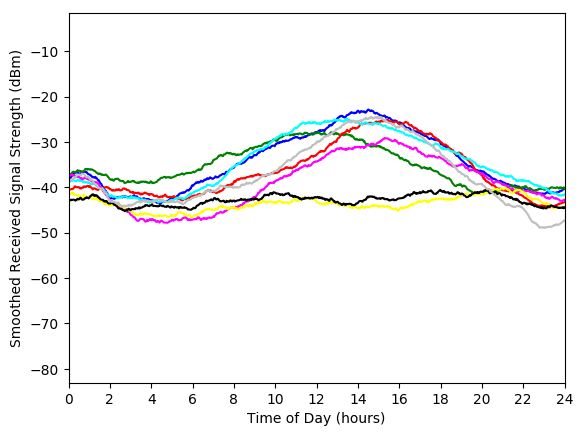
\includegraphics[scale=0.7]{images/2_4_GHz/cot-node12-student_2017-05-22_chan1_image.png}
\end{figure}
\clearpage
Each line/color represents a day, the legend is the following (will be the same for every graph unless indicated otherwise):
\begin{itemize}
\setlength\itemsep{-0.4em}
\item Blue: Monday, May 15th	
\item Green: Tuesday, May 16th
\item Red: Wednesday, May 17th
\item Cyan: Thursday, May 18th
\item Magenta: Friday, May 19th
\item Yellow: Saturday, May 20th
\item Black: Sunday, May 21st
\item Grey: Monday, May 22nd
\end{itemize}
Looking at the spectrum with all the channels as a whole proved not very useful when assessing the state of the spectrum because the if one of the non-overlapping channels is busy it would sway the graph to reflect the entire band to be busy, which would not be the case.
\section{Findings}
\subsection{Evolution throughout the day}

\subsection{Recurring patterns between days} 
On the different nodes we had varying degrees of success in finding recurring patterns. In the 2.4 GHz band, two nodes that clearly showed repeating patterns across several days were cot-node8-student and cot-node12-student. Both of these nodes detected patterns, node8 detecting a large increase in spectrum usage in the afternoon and node12 detecting an increase during the daytime on weekdays, while on the weekends there was no increase present. 
\begin{figure}[!htb]
    \centering
    \textbf{CoT-node12-student, channel 1, 15/05 - 22/05}\par\medskip
	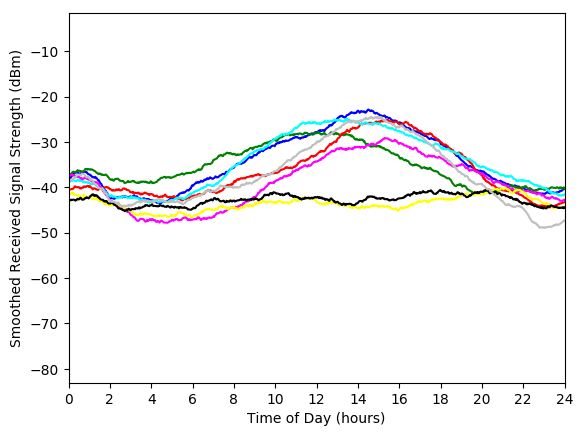
\includegraphics[scale=0.5]{images/2_4_GHz/cot-node12-student_2017-05-22_chan1_image.png}
\end{figure}
\begin{figure}[htb!]
    \centering
    \textbf{CoT-node8-student, channel 1, 12/05 - 16/05}\par\medskip
	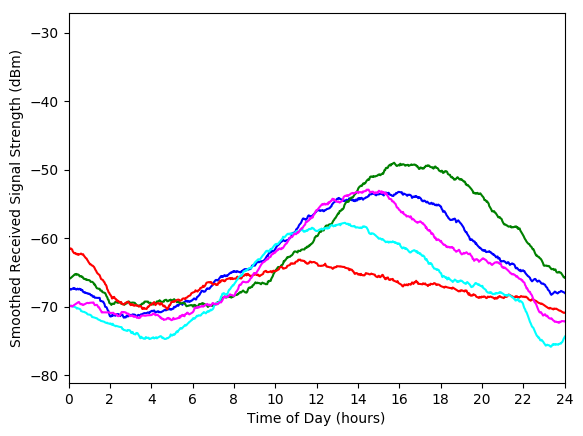
\includegraphics[scale=0.5]{images/2_4_GHz/cot-node8-student_2017-05-16_chan1_image.png}
\end{figure}
\\
For the second graph, belonging to cot-node8-student, we had to change the days because we did not receive all the measurements due to (presumed) hardware failure. For this graph, the legend is: 
\begin{itemize}
\setlength\itemsep{-0.4em}
\item Blue: Friday, May 12th	
\item Green: Saturday, May 13th
\item Red: Sunday, May 14th
\item Cyan: Monday, May 15th
\item Magenta: Tuesday, May 16th
\end{itemize}
Aside from this, for the 2.4GHz band another thing that kept recurring daily was the perceived business of the spectrum on channel 1 on both cot-node3-student and cot-node9-student, as seen in the following graphs:
\begin{figure}[h!]
    \centering
    \textbf{CoT-node3-student, channel 1, 15/05 - 22/05}\par\medskip
	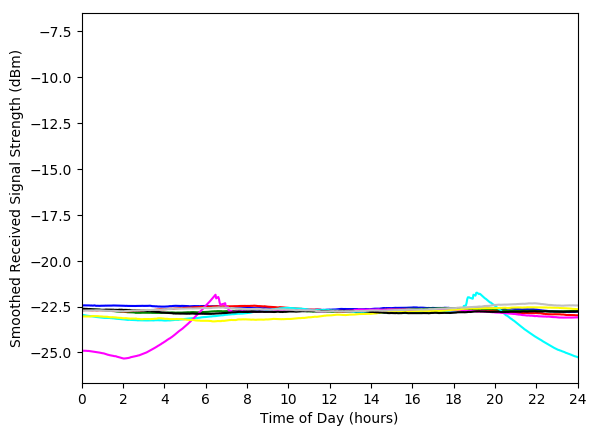
\includegraphics[scale=0.5]{images/2_4_GHz/cot-node3-student_2017-05-22_chan1_image.png}
\end{figure}
\begin{figure}[h!]
    \centering
    \textbf{CoT-node9-student, channel 1, 15/05 - 22/05}\par\medskip
	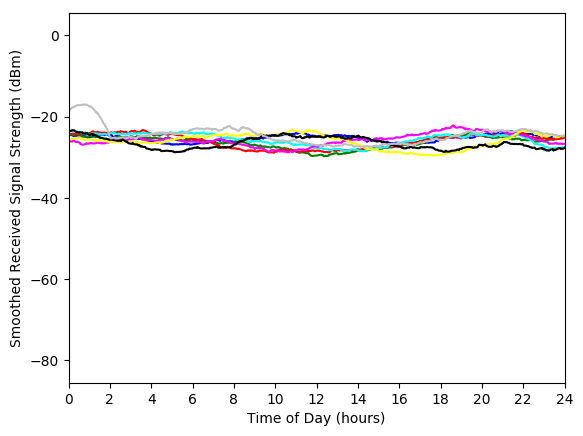
\includegraphics[scale=0.5]{images/2_4_GHz/cot-node9-student_2017-05-22_chan1_image.png}
\end{figure}
and we have included the non pattern-y graphs in the zip file that is included // they are available on demand? TODO) 
<Nodes that have recurring patterns>
\subsection{Calm and busy channels}
As shown in the previous two graphs, channel 1 is usually the most busy channel in the 2.4 GHz band, with channels 6 and 11 trailing far behind. The nodes that saw the most traffic on channel 1 were cot-node3-student and cot-node9-student (see graphs previous subsection) but the traffic they saw on channel 6 and channel 11 is not particulary busy compared to the traffic seen on the other nodes, as we can see from these graphs:\\
\begin{figure}[h!]
    \centering
    \textbf{CoT-node3-student, channel 6, 15/05 - 22/05}\par\medskip
	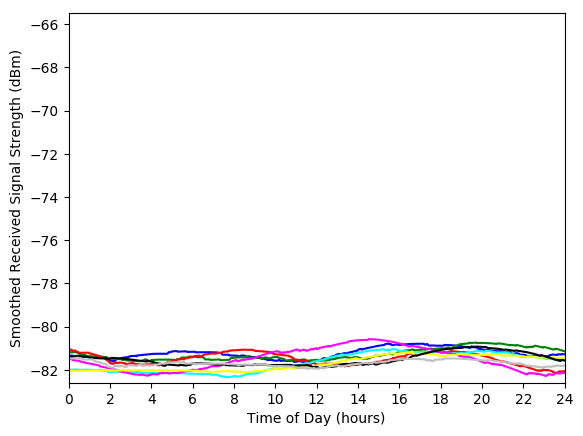
\includegraphics[scale=0.5]{images/2_4_GHz/cot-node3-student_2017-05-22_chan6_image.png}
\end{figure}
\begin{figure}[h!]
    \centering
    \textbf{CoT-node9-student, channel 11, 15/05 - 22/05}\par\medskip
	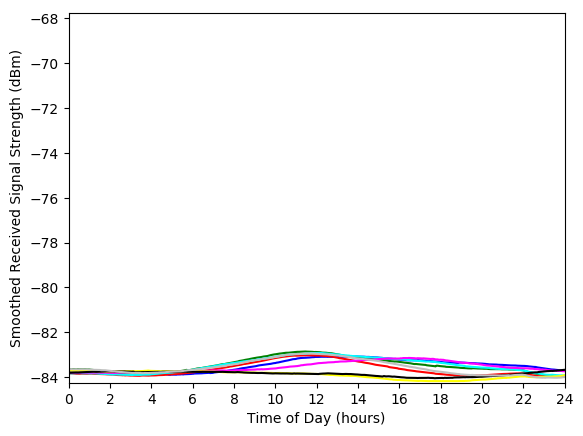
\includegraphics[scale=0.5]{images/2_4_GHz/cot-node9-student_2017-05-22_chan11_image.png}
\end{figure}
\newpage
From the data gathered on the indoors-nodes (i.e. all but node1) we gathered that the 2.4 GHz band's channels 6 and 11 should be usable for these nodes given the amount of traffic we saw on it. The busiest spectrum we saw for the indoor nodes went up to about -75dBm (on cot-node12-student and cot-node3-student). When we compare this to the outdoors node, node1, we see that it's spectrum is also around that value, though slightly higher. For this graph, another legend is used because this node also experienced a (presumed) hardware failure.
\begin{itemize}
\setlength\itemsep{-0.4em}
\item Blue: Saturday, May 13th
\item Green: Sunday, May 14th
\item Red: Monday, May 15th
\item Cyan: Tuesday, May 16th
\item Magenta: Wednesday, May 17th
\end{itemize}
\begin{figure}[h!]
    \centering
    \textbf{node1, channel 6, 13/05 - 17/05}\par\medskip
	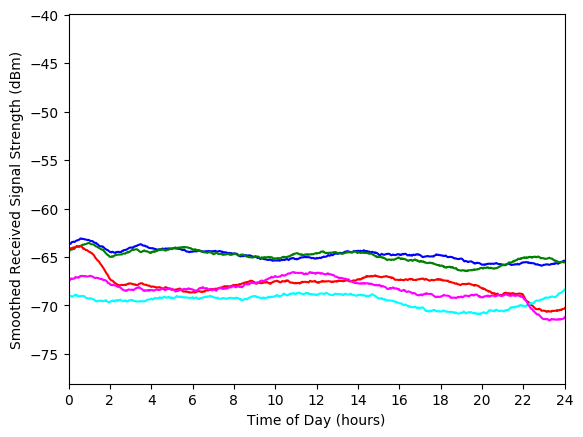
\includegraphics[scale=0.5]{images/2_4_GHz/node1_2017-05-17_chan6_image.png}
\end{figure}
\begin{figure}[h!]
    \centering
    \textbf{node1, channel 11, 13/05 - 17/05}\par\medskip
	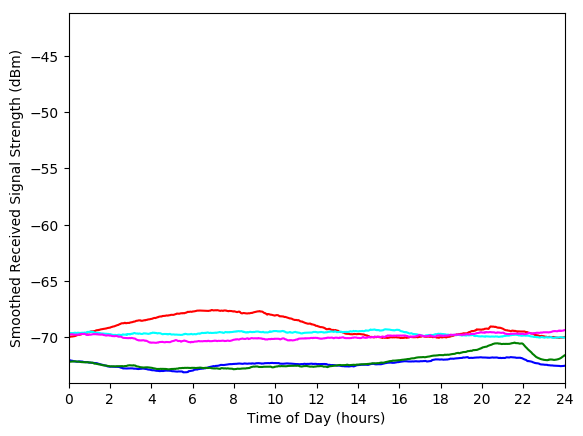
\includegraphics[scale=0.5]{images/2_4_GHz/node1_2017-05-17_chan11_image.png}
\end{figure}
\subsection{2.4 GHz vs 5 GHz}
niks van de 5ghz bevat iets zinnigs (op node3 / chan36 na) - nodes te ver weg ?
>> still running the graph generator for 5GHz to compare lol
\subsection{Validation}
In terms of data validation, we have three parts that we looked at that give us confidence that our data would be valid.
scans met / zonder sturende laptop - stukje had gij al TODO

A second point is the discovering of daily patterns where we expected them. This includes the pattern of daily activity seen in the node at the Middelheim campus as well as seeing a decrease in activity on holidays such as May 1st TODO, we saw this on 12.. 
The third and final point that enforces our trust in the validity of the data we collected and thus also our findings is the fact that the outside node's measurements do not vary wildly from the indoor measurements: it's channel 6 and channel 11 activity is lower than it's channel 1 activity, which is the busiest channel. There is more jitter on the outdoor node's results which is most likely due to it being outside. Our measurements for channel 1 on the outside node can be found below:\\ 
\begin{figure}[h!]
    \centering
    \textbf{node1, channel 1, 13/05 - 17/05}\par\medskip
	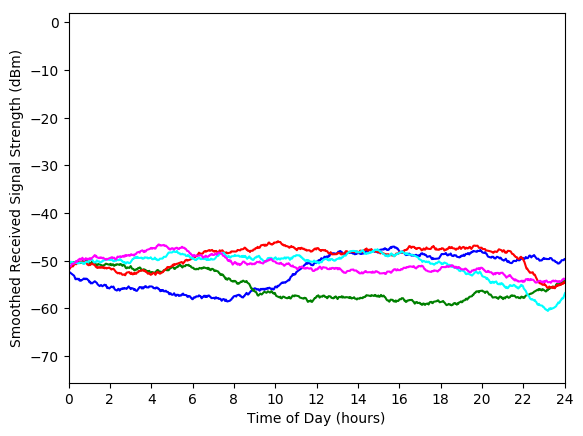
\includegraphics[scale=0.5]{images/2_4_GHz/node1_2017-05-17_chan1_image.png}
\end{figure} \newpage
\section{Conclusions}
So, how bad is it, in general? That was the question to which we sought to find an answer in this project. From the results, it seems clear that the 5 GHz band near the nodes is mostly unused and the 2.4 GHz band could be used if set to chan6 or chan11 TODO

\bibliographystyle{IEEEtran}
\bibliography{IEEEabrv,../chapters/bibliography}




% that's all folks
\end{document}
